% Template for ICASSP-2020 paper; to be used with:
%          spconf.sty  - ICASSP/ICIP LaTeX style file, and
%          IEEEbib.bst - IEEE bibliography style file.
%
% --------------------------------------------------------------------------
\documentclass{article}
\usepackage{spconf,amsmath,graphicx}
\usepackage{amsmath}
\usepackage{amsthm}
\usepackage{amsfonts}
\usepackage{bbm}
\usepackage{ifpdf}
\usepackage{float}
\usepackage{fancyhdr}
\usepackage{xcolor}
\usepackage{multirow}
\usepackage{bm}
\usepackage[toc,page]{appendix}
%\usepackage{cite}

% Example definitions.
% --------------------
\def\x{{\mathbf x}}
\def\L{{\cal L}}

% Title.
% ------
\title{Fast graph kernel with optical random features}
%
% Single address.
% ---------------
\name{ \qquad Hashem Ghanem\qquad Nicolas Keriven \qquad Nicolas Tremblay }

\address{ CNRS, GIPSA-lab, FR-38402 Saint Martin d’Heres Cedex, France}
%
% For example:
% ------------
%\address{School\\
%	Department\\
%	Address}
%
% Two addresses (uncomment and modify for two-address case).
% ----------------------------------------------------------
%\twoauthors
%  {A. Author-one, B. Author-two\sthanks{Thanks to XYZ agency for funding.}}
%	{School A-B\\
%	Department A-B\\
%	Address A-B}
%  {C. Author-three, D. Author-four\sthanks{The fourth author performed the work
%	while at ...}}
%	{School C-D\\
%	Department C-D\\
%	Address C-D}
%
\begin{document}
%\ninept
%
\newtheorem{theorem}{Theorem} 
\maketitle
%
\begin{abstract}
%Graph Classification is the problem of mapping graphs to the classes they belong to.
The graphlet kernel is a classical method in graph classification. In its most generic version, it however suffers from a high computation cost due to the isomorphism test it includes. As a generic proxy, the latter can be replaced with a user-defined mapping that computes various graph characteristics, however usually at the cost of losing information. In this paper, we propose to leverage \emph{kernel random features} within the graphlet framework, and establish a theoretical link with a mean kernel metric. If, at first glance, this method does not necessarily allow to reduce the computational complexity of the graphlet kernel, we then incorporate \emph{optical} random features that can complete such computation in \emph{constant time}. Experiments shows that the resulting algorithm is orders of magnitude faster that the graphlet kernel for the same, or better, accuracy.
\end{abstract}
%
\begin{keywords}
Optical random features, Graph kernels
\end{keywords}
%
\section{Introduction}
\label{sec:intro}
In mathematics and data science, graphs are used to model a set of objects (the \emph{nodes}) and their interactions (the \emph{edges}). %Having \emph{a priori} known graph classes, \emph{graph classification} consists in predicting the class of an entire graph.
Given a set of pre-labeled graphs $(\mathcal{X}=\{\G_1,\ldots,\G_n\}, \mathcal{Y}=\{y_1,\ldots,y_n\})$, where each graph $\G_i$ belongs to the class with label $y_i$, graph classification consists in designing an algorithm that outputs the class label of a new graph.
%
For instance, proteins can be modeled as graphs: amino acids are nodes and the chemical links between them are edges. They can be classified to enzymes and non-enzymes \cite{protein_application}.
%
In social networks analysis, post threads can be modeled with graphs whose nodes are users and edges are replies to others' comment \cite{graph_soc_net}. One task is then to discriminate between discussion-based and question/answer-based threads \cite{class_Reddit}.
% where an edge between two nodes exists if one replies to the other's comment on that thread 
 %For the two examples, , as in the D\&D dataset. In social networks, , as in Reddit-Binary dataset.
%
In addition to the graph structure, nodes and edges may have extra features. While it has been shown that node features are important to obtain high classification performance \cite{node_features}, here we focus on the case where one has only access to the graph structure.%\BlankLine


%\noindent\textbf{Related work.}
Structure-based graph classification has been tackled with many algorithms. Frequent subgraphs based algorithms \cite{frequent_subgraphs} analyze the graph dataset $\mathcal{X}$ to catch the frequent and discriminative subgraphs and use them as features. Kernel-based algorithms \cite{kriege_graph_kernels} can be used by defining similarity functions (kernels) between graphs. An early and popular example is the \emph{graphlet kernel}, which computes frequencies of subgraphs. It is however known to be quite costly to compute \cite{graphlet_kernel}, in particular due to the presence of graph isomorphism tests. While acceleration can be provided in particular cases \cite{Fast_graphlet}, the general case remains open.
Finally, Graph neural networks (GNNs) \cite{GNN_bruna, GNN_review} have recently become very popular in graph machine learning. They are however known to exhibit limited performance when node features are unavailable \cite{GNN_limits}. %Recently, a particular model called GIN (Graph Isomorphism Network) was developed and provided high performance classification.
%\BlankLine

%\noindent\textbf{Contribution:}
In kernel methods, random features are an efficient method to approximate certain kernel functions \cite{Rahimi, RF_1}. Recently, it has been shown that \emph{optical computing} can be leveraged to compute such random features in \emph{constant time} in \emph{any dimension} -- within the limitations of the current hardware, here referred to as Optical Processing Units (OPUs).
%On the other hand, the graphlet kernel represents a graph by how many times graphs of a smaller size occur in it. This kernel includes the isomorphism test in the counting process which makes it computationally expensive.
The main goal of this paper is to provide a proof-of-concept answer to the following question: can leverage OPUs computations be used to reduce the computational complexity of a combinatorial problem like the graphlet kernel? Drawing on a connection with mean kernels and Maximum Mean Discrepancy (MMD) \cite{gretton}, we show, empirically and theoretically, that a fast and efficient graph classifier can indeed be obtained with OPU computations.

\section{Background}
\label{sec:background}
%\subsection{The graphlet kernel}\label{sec:graphlet_kernel}
First, we present the concepts necessary to define the graphlet kernel. We represent a graph of size $v$ by the adjacency matrix $\mathbf{A}\in \{0,1\}^{v\times v}$, such that $a_{i,j} =1$ if there is an edge between nodes $\{i,j\}$ and $0$ otherwise. Two graphs are said to be isomorphic ($\G\cong \G')$ if we can permute the nodes' labels of one such that their adjacency matrices are equal \cite{isomorphism}. 

In this paper, we will, depending on the context, manipulate two different notions of $k$-graphlets: with or without discriminating isomorphism. We denote by $\mathfrak{H}=\{\phlet_1,..., \phlet_{N_k}\}$ the set of all non-isomorphic graphs of size $k$, and $\bar\mathfrak{H}=\{\phlet_1,..., \phlet_{\bar N_k}\}$ with $\bar N_k = 

We define the matching function $\varphi_k^{match}(\mathcal{F}) = \left[ 1_{(\mathcal{F} \cong \phlet_i)}\right]_{i=1}^{N_k} \in \{0,1\}^{N_k}$, where $1_\Omega$ is the indicator function. In words, $\match(\mathcal{F})$ is a Boolean vector of dimension $N_k$ which has a 1 in the coordinate $i$ if $\mathcal{F}\cong \phlet_i$, and $0$ otherwise. 
Let $\mathfrak{F}_\G=\{\mathcal{F}_1,\mathcal{F}_2,\ldots,\}$ be the set of subgraphs induced by all size-k subsets of nodes  in a graph $\G$. We assign each graph with the following representation vector, called k-spectrum:
\begin{equation}
\mathbf{f}_\mathcal{G}=\frac{1}{|\mathfrak{F}_\mathcal{G}|}\sum_{\mathcal{F}\in\mathfrak{F}_\mathcal{G}} \match (\mathcal{F}) \in \R ^{N_k}
\end{equation}
For two graphs $\G,\G'$, the graphlet kernel is defined by the inner product $\bld{f}_\G^T\bld{f}_{\G'}$. The graphlet kernel performs well especially with a sufficiently large value of $k$ \cite{graphlet_kernel}. However, in each graph $\G$ of size $v$, the computation cost to compute $\bld{f}_\G$ is $ C_{gk}= \mathcal{O}\left(\tbinom{v}{k} N_k C^{\cong}_k\right)$, where $C^{\cong}_k$ is the cost of the isomorphism test between two graphs of size $k$. This cost is expensive due to: i/ $\binom{v}{k}$ explodes as $v$ or $k$ increase, ii/ $N_k$ is exponential in $k$, iii/ yet there is no known method to test isomorphism in polynomial time of $k$ \cite{isomorphism_np}. 

Usually, uniform graphlet sampling is used to accelerate the graphlet kernel \cite{graphlet_kernel}, where sampling a size-k subgraph means: first we uniformly at random choose $k$ nodes from the graph, then we sample the subgraph induced by those  nodes. This yields that each sample follow a uniform distribution over $\mathfrak{F}_\G$.

Knowing this, the $k$-spectrum $\bld{f}_\G$ can be interpreted as follows: if one samples a subgraph from $\mathcal{G}$, then one has a probability $(\bld{f}_\G)_i$ of obtaining $\phlet_i$, \emph{i.e.}: $	\label{eq:histo_unif}
	\mathbf{f}_\mathcal{G} = \mathbb{E}_{F \sim {\rm unif}} ~\varphi^{match}_k(F)$. 
	It is thus natural to approach $\mathbf{f}_\mathcal{G}$ with a sample average, where by sampling $s$ subgraphs of size $k$ to form the collection 
$\hat{\mathfrak{F}}_\G=\{F_1,...,F_s\}$, the estimator:
\begin{align}
	\label{eq:fhat_unif}
	\hat{\mathbf{f}}_\mathcal{G} =\frac{1}{s}\sum_{F\in\hat{\mathfrak{F}}_\G} \varphi^{match}_k(F).
\end{align}
verifies by the law of large numbers that $\hat{\mathbf{f}}_\G \xrightarrow[s \to \infty]{} \mathbf{f}_\mathcal{G}$ with probability $1$.

The computation cost per graph of the  graphlet kernel with graph sampling is $C_{gk + gs}= \mathcal{O}\left(s C_S N_k C^{\cong}_k\right)$, where $C_S$ is the cost of sampling one subgraph. Although the term $\binom{v}{k}$ doesn't exist  in this cost, still for a specific certainty in estimating $\bld{f}_\G$, the required number of samples $s$ must be proportional to $N_k$ \cite{graphlet_kernel}. So this version is still expensive especially when $k$ is large. 

In fact, there exist many different sampling techniques $S_k$, each follows a specific random process in sampling the $k$ nodes from a graph $\G$. As a result, subgraphs sampled with a technique different from the uniform sampling will have a different histogram $\bld{f}_{\G,S_k}$ than the one defined by $\bld{f}_\G$ \cite{leskovec2006sampling}. Such sampling technique is the random walk (RW) sampler. Unlike uniform sampling, RW tends to sample connected  subgraphs, which are more informative about the graph structure. 


\iffalse
\subsection{Kernel Random features}\label{sec:Random_features}
Kernels by definition are symmetric and positive  semi-definite functions that takes two data points as input. Based on Mercer theorem, for each kernel $\kappa$, there exists a Hilbert space $\mathbb{H}$ and a  feature map $\phi:\mathbb{R}^d\mapsto\mathbb{H}$ such that:  
	\begin{equation}
	\label{eq:kernel_main_equation}
	\kappa(\mathbf{x},\mathbf{x}')=<\phi(\mathbf{x}),\phi(\mathbf{x}')>_\mathbb{H},~ \forall \mathbf{x},\mathbf{x}'\in\mathbb{R}^d
	\end{equation}
	where $<\phi(\mathbf{x}),\phi(\mathbf{x}')>_\mathbb{H}$ is the inner product defined in $\mathbb{H}$.

Random features (RF) is an approach developed to approximate kernels with reduced computational time  \cite{rahimi2008random}. The idea is that, instead of considering the true lifting function $\phi$ in Eq. \ref{eq:kernel_main_equation}, we explicitly map the data points using an appropriate randomized feature map $\varphi:\mathbb{R}^d \xrightarrow{}\mathbb{C}^m$, such that the kernel for two data points $\mathbf{x}, \mathbf{x}'$ is approximated by the inner product of their random features with high probability:
\begin{equation}
\label{eq:approx_RF}
\kappa(\mathbf{x},\mathbf{x}')=<\phi(\mathbf{x}),\phi(\mathbf{x}')>_\mathbb{H} \approx \varphi(\mathbf{x})^*\varphi(\mathbf{x}')
\end{equation}
where $^*$ stands for the conjugate transpose. Most RF constructions are known as Random Fourier Features (RFF), and are based on
the following theorem.
\begin{theorem}[Bochner's theorem]
	A continuous and shift-invariant kernel $\kappa(\mathbf{x},\mathbf{x}')=\kappa(\mathbf{x}-\mathbf{x}')$ on $\mathbb{R}^d$ is positive definite if and only if $\kappa$ is the Fourier transform of a non-negative measure.
\end{theorem}
Therefore, scaling such kernels to obtain $\kappa(0) = \int p = 1$,   its Fourier transform $p(\mathbf{w})$ becomes a correct probability distribution, so we write:
\begin{equation}
\label{eq:real_Fourier_integral}
\kappa(\mathbf{x}-\mathbf{x}')=\int_{\mathbb{R}^d}p(\mathbf{w})cos({\mathbf{w}^T(\mathbf{x}-\mathbf{x}')})d\mathbf{w}=E_{\mathbf{w}\sim p}[ \xi_\mathbf{w}(\mathbf{x}) \xi_\mathbf{w}(\mathbf{x}')]
\end{equation}
where $ \xi_\mathbf{w}(\mathbf{x})=\sqrt{2}cos(\mathbf{w}^T\mathbf{x}+b)$ such that $\mathbf{w}$ is drawn from $p$ and $b$ is drawn uniformly from $[0,2\pi]$. The RF methodology consists in averaging $m$ instances of $\  \xi_\mathbf{w}(\mathbf{x})^*  \xi_\mathbf{w}(\mathbf{x}')$  with different random frequencies $\mathbf{w}_j$ drawn identically and independently (iid) from $p$, that is, define
\begin{align}
	\label{eq:def_RF}
	\varphi(\mathbf{x}) = \frac{1}{\sqrt{m}} ( \xi_{\mathbf{w}_j}(\mathbf{x}) )_{j=1}^m \in \mathbb{C}^m
\end{align}
such that $\varphi(\mathbf{x})^*\varphi(\mathbf{x}')=\frac{1}{m} \sum_{j=1}^m \xi_{\mathbf{w}_j}(\mathbf{x})^*\xi_{\mathbf{w}_j}(\mathbf{x}')$, which, by Hoeffding's inequality, converges exponentially in $m$ to $\kappa(\mathbf{x},\mathbf{x}')$.
\fi

\section{Method} \label{ssed to get a lowerec:pagestyle}
\subsection{Proposed algorithm}
\label{sec:algo}
\begin{algorithm}[h]
\DontPrintSemicolon
  \KwInput{labeled graph dataset $\mathcal{X}=(\G_i,y_i)_{i=1,\ldots,n}$}
  \tools{Graphlet sampler $S_k$, a function $\varphi$, linear classifier (ex. SVM) }\\
  \Hyp{k: graphlet size, $s$: number of graphlet samples per graph}, $m$: \emph{number of random features}\\
  \KwOutput{Trained model to classify graphs}
  
  %\KwData{Testing set $x$}
  %$\sum_{i=1}^{\infty} := 0$ \tcp*{this is a comment}
  %\tcc{}
  \Algo{\\}
  Random initialization of the SVM weights\\
  \For{$\G_i$ in $\mathcal{X}$}{
  $\mathbf{z}_i=\mathbf{0}$ (null vector of size $m$) \\
  \For{$j=1:s$}{
  $F_{i,j}\gets S_k(\G_i)$\\
  $\mathbf{z}_i\gets \mathbf{z}_i +\frac{1}{s}\varphi(F_{i,j})$
  }
  }
  $\mathcal{D}_{\varphi}\gets (\mathbf{z}_i,y_i)_{i=1,\ldots, n}$\\
  Train the linear classifier on the new vector-valued dataset $\mathcal{D}_{\varphi}$
\caption{GSA-$\varphi$ generic algorithm}
\end{algorithm}

 We propose to replace $\match$ with a user-defined map $\varphi$, and to replace the uniform sampler with a user-chosen one like the RW sampler.  This makes it possible to deploy the OPU technology with this algorithm. We refer to this framework as \emph{graphlet sampling and Averaging $GSA-\varphi$}, and its cost per graph for a specific $\varphi$ is $C_{GSA-\varphi}= \mathcal{O}\left(s C_S C_{\varphi}\right)$, where $C_{\varphi}$ is the cost of applying $\varphi$ on one graphlet. 

The function $\varphi$ here maps each subgraph to an $m$-dimensional space $\mathbb{R}^m$. Note that choosing $\varphi = \match$ and $S_k$ as the uniform sampler, GSA-$\match$ turns out to be the  graphlet kernel with graphlet sampling.  We see next that choosing  $\varphi$ as random maps is both fast and efficient.

\subsection{Efficiency of kernel random features with $GSA-\varphi$} 
\label{sec:MMD}
A kernel $\kappa$ associated to a random features (RF) decomposition is a positive definite function of two inputs that can be decomposed  as follows   \cite{rahimi2008random}:
\begin{equation}
\label{eq:RF_decomposition}
\kappa(\mathbf{x},\mathbf{x}')=\mathbb{E}_{\mathbf{w}\sim p}[ \xi_\mathbf{w}(\mathbf{x}) \xi_\mathbf{w}(\mathbf{x}')]
\end{equation}
where $\mathbb{E}$ stands for the expectation, $p$ is a probability distribution, and $\xi$ is a function parameterized by $\mathbf{w}$. 
To approximate such kernels, we can emperically average $m$ realizations of $\xi_\mathbf{w}(\mathbf{x}) \xi_\mathbf{w}(\mathbf{x}')$. To do that, we define RF maps:
\begin{equation}
	\label{eq:def_RF}
	\varphi(\mathbf{x}) = \frac{1}{\sqrt{m}} ( \xi_{\mathbf{w}_j}(\mathbf{x}) )_{j=1}^m \in \mathbb{C}^m
\end{equation}
where  $m$ is called here the number of features and the frequencies $\mathbf{w}_j$ are drawn identically and independently (iid) from $p$. Then, $\kappa(\mathbf{x},\mathbf{x}')\approx	\varphi(\mathbf{x})^T	\varphi(\mathbf{x}')$.

 For each kernel as in  \eqref{eq:RF_decomposition} , and for any two graphs $\G,\G'$, we define the MMD (Maximum Mean Discrepancy) metric between the two corresponding distrubutions  $\bld{f}_{\G,S_k}, \bld{f}_{\G',S_k}$ by:
 \[
 MMD^2(\bld{f}_{\G,S_k}, \bld{f}_{\G',S_k}) = \mathbb{E}_{\mathbf{w}} \Big( \left| \mathbb{E}_{S_k(\G)} \xi_\mathbf{w}(F) - \mathbb{E}_{S_k(\G')} \xi_\mathbf{w}(F') \right|^2 \Big)
 \]
 The main property of the MMD is that, for so-called \emph{characteristic kernels}, it is a true metric on distributions, \emph{i.e.} $MMD(\mathcal{P}, \mathcal{Q}) = 0 \Leftrightarrow \mathcal{P} = \mathcal{Q}$. In addition, most usual kernels, like the Gaussian kernel, are characteristic \cite{MMD}.
 
 The next theorem shows the efficiency of using RF maps as in \eqref{eq:def_RF} with our algorithm. It states  that the Euclidean distance between the representation vectors $\bld{z}_\G, \bld{z}_{\G'}$ converges to the MMD metric between their distributions $\bld{f}_{\G,S_k}$, $\bld{f}_{\G',S_k}$. 



\begin{theorem}\label{theorem:concentration}
Let $\G$ and $\G'$ be two graphs, $\mathfrak{F}_\G=\{F_i\}_{i=1}^{s}$ (resp. $\mathfrak{F}_{\G'}=\{F_i'\}_{i=1}^{s}$) be $iid$ size-k graphlet samples drawn from $S_k(\G)$ (resp. $S_k(\G')$). Assume a random feature map as in \eqref{eq:def_RF}. Assume that $|\xi_\mathbf{w}(F)| \leq 1$ for any $\mathbf{w},F$.
We have for all $\delta>0$ and with probability at least $1-\delta$:
\begin{align*}
 \Big|\|\varphi(\mathfrak{F}_\G) - \varphi(\mathfrak{F}_{\G'})\|^2 - MMD(\bld{f}_{\G,S_k},\bld{f}_{\G',S_k})^2 \Big| \leq \\\frac{4 \sqrt{\log (6/\delta)}}{\sqrt{m}} + \frac{8\left(1+\sqrt{2\log(3/\delta)}\right)}{\sqrt{{s}}}
\end{align*}
\end{theorem}

\begin{proof}
 see Appendix.
\end{proof}

\subsection{Considered choices of $\varphi_{RF}$}
\label{sec:phi_choices}
\textbf{Gaussian maps $\boldsymbol{\varphi_{Gs}}$ applied on the adjacency matrix}: $\varphi_{Gs}$ is the RF map of the Gaussian kernel \cite{rahimi2008random}. We for each subgraph $\F$ take its vectorized adjacency matrix  $\mathbf{a}_\F=flatten(\mathbf{A}_\F)$ as input. Then:
\begin{equation}
\label{eq:Gaussian_map}
    \varphi_{Gs}(\F) = \frac{1}{\sqrt{m}} \left( \sqrt{2} \cos(\mathbf{w}_j^T\mathbf{a}_\F+b_j) \right)_{j=1}^m \in \mathbb{R}^m
\end{equation}
where the frequencies $\mathbf{w}_j\in \R^{k^2}$ are drawn from a Gaussian distribution with the inverse variance of the original kernel. 
\BlankLine
\noindent\textbf{Gaussian maps $\boldsymbol{\varphi_{Gs+Eig}}$ applied on the sorted eigenvalues of the adjacency matrix:} instead of passing the vectorized adjacency matrix as input, we pass the vector of its sorted eigenvalues $\bm{\lambda}\in\R^k$. The motive proposing $\varphi_{Gs+Eig}$ is that it respects the isomorphism test since: 
i/ $\bld{\lambda}(\bld{A})=\bld{\lambda}(\bld{PAP^T})$ for any permutation matrix $\bld{P}$, 
ii/ $F\cong F' \Rightarrow\exists \bld{P}, \bld{A}_F=P\bld{A}_{F'}P^T$.  
Thus, $F\cong F' \Rightarrow \varphi_{Gs+Eig}(F)=\varphi_{Gs+Eig}(F')$. $\varphi_{Gs+Eig}$ maps isomorphic subgraphs to the same point in $\R^m$.
\BlankLine
\noindent\textbf{Optical random feature maps $\varphi_{OPU}$:} This corresponds to the fastest version of our algorithm. OPUs (Optical Processing Units) technology was developed to compute  a specific random features mapping in \emph{constant time  $\mathcal{O}(1)$} in both $m$ and $k$ using light scattering \cite{saade_opu}. Having the random matrix $\bld{W}$, traditional random maps (ex. $\varphi_{Gs}$) need  $\mathcal{O}(mk^2)$ cost to compute $\bld{Wx}$ as in \eqref{eq:Gaussian_map}. An OPU computes its associated map at the speed of light, this map is modeled as follows \cite{saade_opu}:
\[
\label{OPU_equation}
\mathbf{\varphi}_{OPU}(\mathbf{x})=|\mathbf{Wx+b}|^2 ;~\mathbf{W}\in \mathbb{R}^{m\times d},\mathbf{b}\in \mathbb{R}^m, \mathbf{x}\in \mathbb{R}^d
\]
Where $\mathbf{b}$ is a random bias vector, $d$ is the input space dimension, the amplitude function $|\cdot|$ is taken element wise, and $\mathbf{W}$ is a random \emph{iid} complex matrix with Gaussian real and imaginary parts.
The complexities of the different mappings $\varphi$ examined in this work are summarized in Table \ref{tab:cost}.



\begin{table}
\centering
\begin{tabular}{|c|c|c|}
\hline
\multicolumn{2}{|c|}{Graphlet kernel} & $O(\tbinom{v}{k} N_k C^{\cong}_k)$\\ \hline \hline
%
\multirow{4}{*}{GSA-$\varphi$ with:} & $\varphi^{match}_k$ & $O(C_s s N_k C^{\cong}_k)$ \\
& $\varphi_{Gs}$ & $O(C_s s m k^2)$ \\ 
& $\varphi_{Gs+Eigen}$  & $O(C_s s (m k + k^3))$ \\ 
& $\varphi_{OPU}$  & $O(C_s s)$ \\ \hline
\end{tabular}
\caption{Per-graph complexities of GSA-$\varphi$.}
\label{tab:cost}
\end{table}


\section{Experiments}\label{sec:experiments}
\subsection{Setup}\label{sec:setup}
With respect to the performance and  the computation cost, we compare different choices of  map $\varphi$ in $GSA-\varphi$. We benchmark the performance of $GSA-\varphi_{OPU}$ against GIN based graph convolutional network.

In all experiments except the last one, we use a synthetic dataset generated by a \emph{Stochastic Block Model (SBM)} \cite{SBM}. We generate $300$ graphs, $240$ for training  and $60$ for testing. Each graph has $v=60$ nodes divided equally between six communities. Moreover, graphs are divided into two classes $\{0 , 1\}$ based on the edges distribution considered. For each class we fix two values $(p_{in} , p_{out})$ which are  the probabilities of generating an edge between any two nodes when they are in the same community and when they are in different ones, respectively. Besides, to prevent the classes from being easily discriminated by the average degree, the pairs $(p_{in,i} , p_{out,i})_{i=0,1}$ are chosen such that all nodes have a fixed expected average degree equal to $10$. Having one degree of freedom left, we fix $p_{in,1}=0.3$, and we vary $r=(p_{in,1}/p_{in,0})$ the inter-class similarity parameter: the closer $r$ is to $1$, the more similar both classes are, and thus the harder it is to discriminate them.

On the other hand, D\&D is a labeled dataset of size $n=1178$ protein graphs \cite{DD_ref}. Also, nodes have 7 features each, which are not used by our algorithms, \emph{i.e.} we will try to classify the graphs just based on their structure. In what follows, unless otherwise indicated, we use uniform sampling and the adjacency matrix of subgraphs as input.

\begin{figure}[h]
%
\begin{minipage}[b]{.48\linewidth}
  \centering
  \centerline{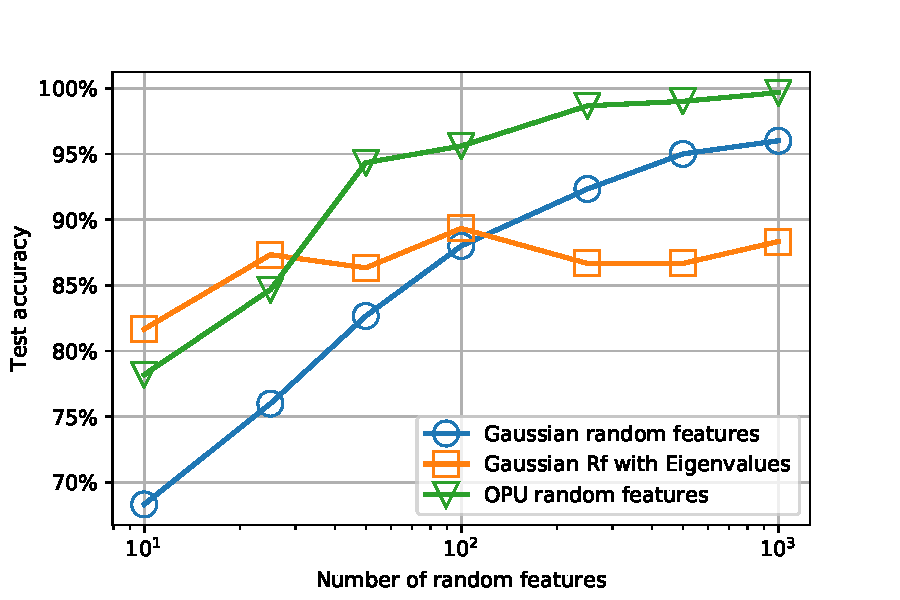
\includegraphics[width=4.3cm]{figs/phi_comparison.pdf}}
%  \vspace{1.5cm}
  \centerline{(a) RF maps}\medskip
  \label{subfig:RF_maps}
\end{minipage}
\hfill
\begin{minipage}[b]{0.48\linewidth}
  \centering
  \centerline{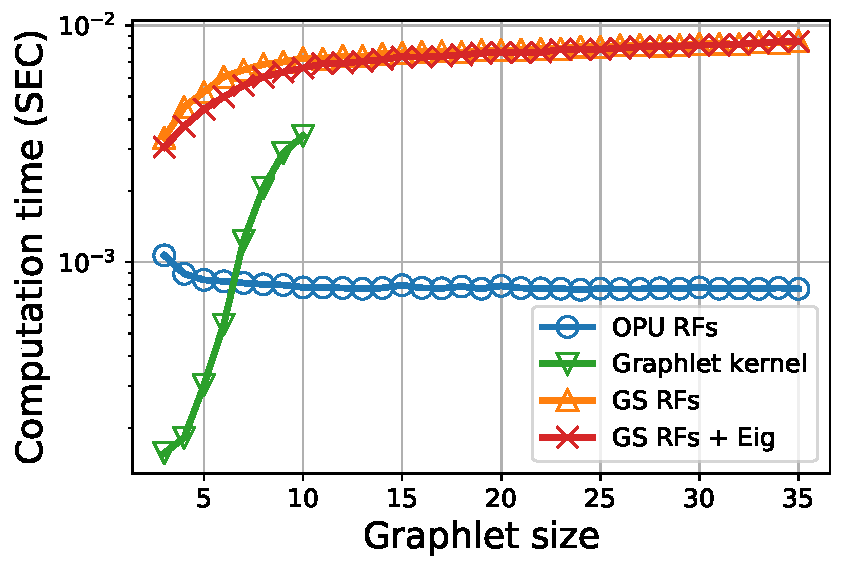
\includegraphics[width=4.3cm]{figs/computational_comp.pdf}}
%  \vspace{1.5cm}
  \centerline{(b) Computation cost}\medskip
\end{minipage}
%
\caption{Comparing different $\varphi$ maps in $GSA-\varphi$. (a) test accuracy when using RF maps with $k=6$ while varying $m$. (b) test accuracy of $GSA-\varphi_{OPU}$ and $GSA-\match$  fixing $k=5$ while varying $r$. (c) Computation time as a function of $k$. If not specified:  $r=1.1$, $s=2000$, $m=5000$ and the Gaussian map variance $\sigma^2=0.01$.}
\label{fig:diff_phi}
%
\end{figure}

\subsection{Choice of feature map $\varphi$}
\textbf{Comparison of random features}: Fig \ref{fig:diff_phi}(a) shows  that $GSA-\varphi_{OPU}$ applied on adjacency matrices gives better test accuracy with sufficiently large $m$ than both $GSA-\varphi_{Gs}$ applied on adjacency matrices or $GSA-\varphi_{Gs+Eig}$ applied on its sorted eigenvalues. On the contrary, $GSA-\varphi_{Gs+Eig}$ performs best with a low number of random features, but increasing this number does not really improve the result and it is over-matched at high $m$. A possible justification is that the eigenvalues of the adjacency matrix lose information about the subgraphs, even though respecting the isomorphism means that we are working with a smaller histogram and less random features are required.

\noindent\textbf{Comparing $GSA-\varphi_{OPU}$ to $GSA-\match$:} from Fig \ref{fig:diff_phi}(b) we observe that  with the same limited number of samples $s$, $GSA-\varphi_{OPU}$ clearly outperforms the approximated graphlet kernel $GSA-\match$, so we conclude that $GSA-\varphi_{OPU}$ is more adapted in this case than the traditional graphlet kernel.

\noindent\textbf{Computational time:} Fig \ref{fig:diff_phi}(c) shows the computation time of each of the previous methods with respect to the subgraphs size $k$. Other parameters are identically fixed for all methods. As expected, the execution time of the approximated graphlet kernel grows exponentially with  $k$, and is polynomial for $GSA-\varphi_{Gs}$ and $GSA-\varphi_{Gs+Eig}$. On the contrary, it is almost constant for $GSA-\varphi_{OPU}$. We point out here that, with the current settings, there is a significant overhead between the point in time where we run our optimizer code on the OPUs server and the point when the OPU  launches the computation. To be fair, this overhead time should be measured and subtracted from $GSA-\varphi_{OPU}$ computation time. As the technology comes into maturity, we can expect this additional time to be significantly reduced. 

To summarize, $GSA-\varphi_{OPU}$ outperforms the traditional methods both in accuracy and computational cost.

% Below is an example of how to insert images. Delete the ``\vspace'' line,
% uncomment the preceding line ``\centerline...'' and replace ``imageX.ps''
% with a suitable PostScript file name.
% -------------------------------------------------------------------------

\subsection{Comparing $GSA-\varphi_{OPU}$ against GIN model}\label{sec:vs_GIN}

In Fig \ref{fig:GCN}, we observe that for subgraphs sizes $>5$, both RW and uniform sampling perform similarly well in $GSA-\varphi_{OPU}$, but RW sampling, as expected, provide more consistent results when the graphlet size $k$ varies. Thus RW sampling is considered in this comparison.
We see that $GSA-\varphi_{OPU}$ with RW  performs better than the GIN model when the graphlet size is greater than 4. We note that we do not report the computational time for GIN, since it is highly dependent on high-speed graphical processing units (GPUs) to do the training process.

\begin{figure}[h]
%
\begin{minipage}[b]{.48\linewidth}
  \centering
  \centerline{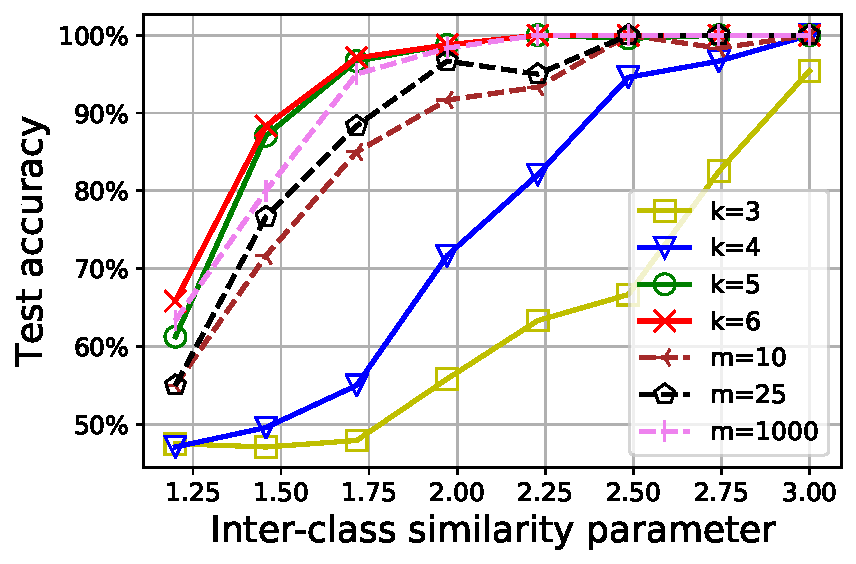
\includegraphics[width=4.3cm]{figs/LightOn_adj_SBM_Similarity_graphlet_size.pdf}}
%  \vspace{1.5cm}
  \centerline{(a) $\varphi_{OPU}$\& uniform sampling}\medskip
\end{minipage}
\hfill
\begin{minipage}[b]{0.48\linewidth}
  \centering
  \centerline{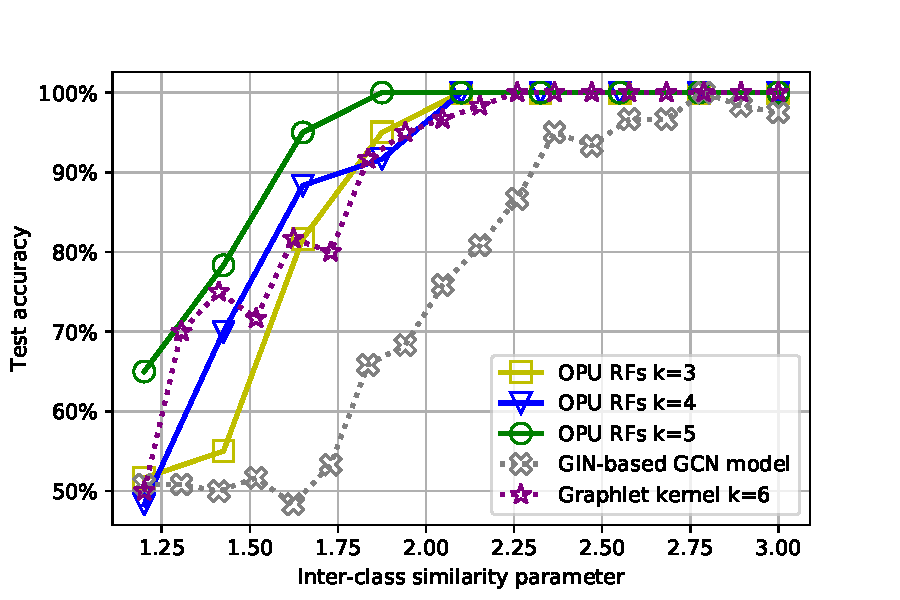
\includegraphics[width=4.3cm]{figs/LightOn_adj_SBM_similarity_graphlet_size_RW.pdf}}
%  \vspace{1.5cm}
  \centerline{(b) $\varphi_{OPU}$\& RW sampling}\medskip
\end{minipage}
%
\caption{Comparing test accuracies of $GSA-\varphi_{OPU}$ and GIN-based GCN network when varying the problem difficulty $r$. We used $GSA-\varphi_{OPU}$ with uniform sampling in (a) and with random walk sampling in (b). In both cases: $s=2000$ and $m=5000$. (c) The model consists of 5 GIN layers then 2 fully connected layers, the dimensions of hidden layers: 4.}
\label{fig:GCN}
%
\end{figure}


\begin{figure}[h]
%
\begin{minipage}[b]{.48\linewidth}
  \centering
  \centerline{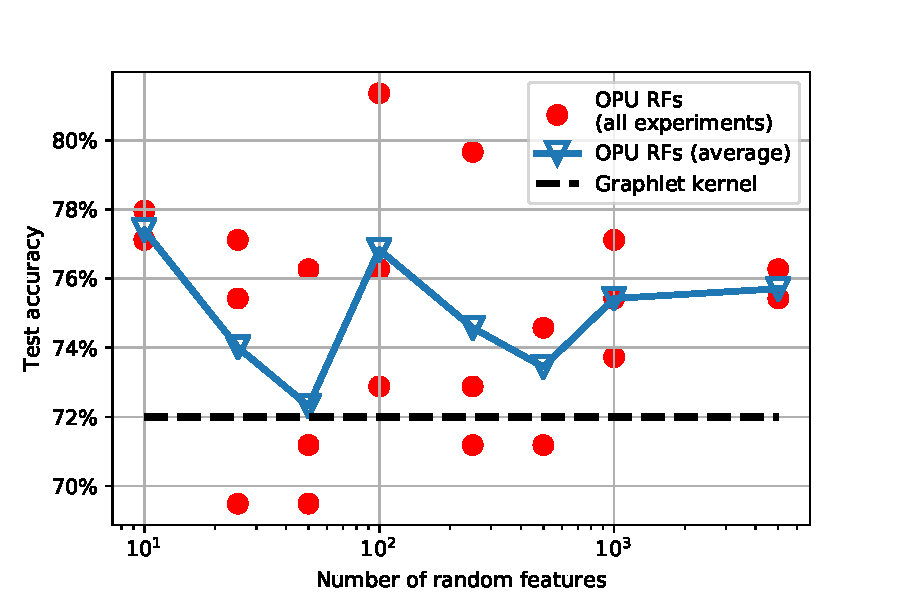
\includegraphics[width=4.3cm]{figs/DD.pdf}}
%  \vspace{1.5cm}
  \centerline{(a) D\&D }\medskip
  \label{subfig:RF_maps}
\end{minipage}
\hfill
\begin{minipage}[b]{0.48\linewidth}
  \centering
  \centerline{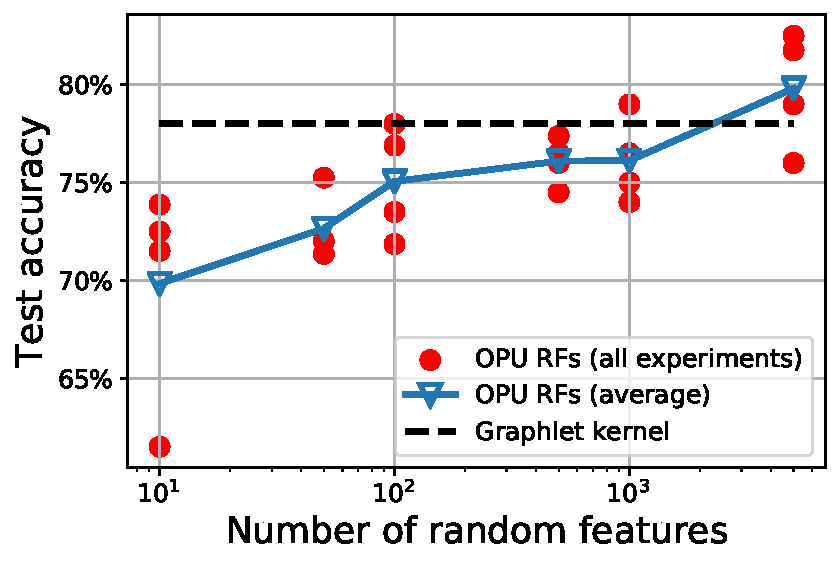
\includegraphics[width=4.3cm]{figs/Reddit.pdf}}
%  \vspace{1.5cm}
  \centerline{(b) Reddit-Binary}\medskip
\end{minipage}
%
\caption{Bench-marking $GSA-\varphi$ against the graphlet kernel as a performance reference on real datasets with: s=4000,k=.}
\label{fig:DD}
%
\end{figure}
In Fig \ref{fig:DD}, we have the test accuracy with varying value of $m$ and fixed $s=4000$, $k=7$. For each value of $m$ we conduct the experiment 5 times and take the average accuracy. Although we do not observe a clear, steady average improvement in accuracy when $m$ grows, the results of the 5 corresponding experiments get more concentrated around the average value, giving a desirable reduced variance between experiments. On the other hand,  accuracy results at low $m$ show high variance between experiments, which might be accentuated by the fact that nodes features are ignored. However, using node features is without doubt necessary to reach state-of-the-art results, and it is an open question how to incorporate that in our algorithm, but our goal here is mainly to test our algorithm on real data as a proof of concept.


% To start a new column (but not a new page) and help balance the last-page
% column length use \vfill\pagebreak.
% -------------------------------------------------------------------------
%\vfill
%\pagebreak

\section{Conclusion}
\label{sec:Conclusion}
We proposed a family of algorithms that combines graphlet sampling with efficient mappings. Then, we proposed to choose this mapping as kernel random maps, and showed a concentration of the random embedding around the MMD metric. Finally, while classical random features still require expensive matrix-vector multiplication, we used optical random features projections, which can be computed in $\mathcal{O}(1)$ to get the algorithm's fastest version. Our Experiments showed that it is significantly faster than traditional graphlet kernel and generally performs better while concentrating around the MMD metric. In our settings, it even outperformed a particular graph convolutional network on graph classification.

 A major point left open to be analyzed is how to use our algorithm to classify graphs with node features. One promising possibility is to use our algorithm to generate features embeddings on the graph level, and then feed these embeddings with the nodes' features to a deep neural network. Doing this, we take advantage of the speed of both our algorithm and GPUs. On the theoretical side, the properties of the MMD metric could be further analyzed on particular models of graphs to get a concentration with higher certainty. 




% References should be produced using the bibtex program from suitable
% BiBTeX files (here: strings, refs, manuals). The IEEEbib.bst bibliography
% style file from IEEE produces unsorted bibliography list.
% -------------------------------------------------------------------------
\bibliographystyle{IEEEbib}
\bibliography{strings,refs}
\begin{appendices}
\section{Proof of Theorem 1}\label{app:proof}
\begin{proof} We decompose the proof in two steps.

\textbf{Step 1: infinite $s$, finite $m$.} First we define the random variables $x_j=| \mathbb{E}_{F \sim S_k(\G)} \xi_{\mathbf{w}_j}(F) - \mathbb{E}_{F' \sim S_k(\G')} \xi_{\mathbf{w}_j}(F') |^2$, which are: i/independent, ii/have expectation $MMD(\G,\G')^2$, /iii are bounded by the interval $[0,4]$ based on our assumption $|\xi_w|\leq 1$. Thus, as a straight result of applying  Hoeffding's inequality with easy manipulation: with probability $1-\delta$
\begin{equation}
\label{eq:step1}
\Big|\frac{1}{m} \sum_{j=1}^m x_j- MMD(\G,\G')^2 \Big| \leq\\ \frac{4 \sqrt{\log (2/\delta)}}{\sqrt{m}}
\end{equation}

\textbf{Step 2: finite $s$ and $m$.} For any \emph{fixed} set of random features $\{w_j\}_{1,\ldots,m}$ and based on our previous assumptions we have: i/ $\varphi_{RF}$ is in a ball of radius $M=\frac{\sqrt{m}}{\sqrt{m}}=1$, ii/ $ \mathbb{E}_{F \sim S_k(\G)}~ \varphi(F)= \mathbb{E}\left(~\frac{1}{{s}} \sum_i \varphi(F_i)~\right)$. Therefore, we can directly apply the vector version of Hoeffding's inequality on the vectors $\frac{1}{{s}} \sum_i \varphi(F_i)$ to get that with probability $1-\delta$:
\begin{equation}
    \label{eq:fixed_w}
    \left\|\mathbb{E}_{F \sim S_k(\G)} \varphi(F)-~\frac{1}{s} \sum_i \varphi(F_i)~\right\|\leq \frac{1+\sqrt{2\log\frac{1}{\delta}}}{\sqrt{{s}}}
\end{equation}
\vfill\pagebreak
Defining $J_{exp}(\G,\G')=\| \mathbb{E}_{F \sim S_k(\G)} \varphi(F) - \mathbb{E}_{F' \sim S_k(\G')} \varphi(F')\|$ and $J_{avg}(\G,\G')=\| \frac{1}{{s}} \sum_i \varphi(F_i) - \frac{1}{{s}} \sum_i \varphi(F'_i)\|$, then using triangular inequality followed by a union bound based on \eqref{eq:fixed_w}, we have the following with probability $1-2\delta$,
\begin{align*}
    \Big | J_{exp}(\G,\G') - J_{avg}(\G,\G')\Big | \leq \frac{2}{\sqrt{{s}}}\left(1+\sqrt{2\log\frac{1}{\delta}}\right)
\end{align*}

On the other hand, $ J_{exp}(\G,\G') + J_{avg}(\G,\G')\leq 4$, so with same probability:
\begin{equation}\label{eq:step2}
    \Big | J_{exp}(\G,\G')^2 - J_{avg}(\G,\G')^2 \Big | \leq \frac{8}{\sqrt{{s}}}\left(1+\sqrt{2\log\frac{1}{\delta}}\right)
\end{equation}
Since it is valid for any fixed set of random features, it is also valid with \emph{joint} probability on random features and samples, by the law of total probability.

Finally, combining \eqref{eq:step1}, \eqref{eq:step2} with a union bound and a triangular inequality, we have with probability $1-3\delta$,
\begin{align*}
\Big|\|\varphi(\mathfrak{F}_\G) - \varphi(\mathfrak{F}_{\G'})\|^2 - MMD(\G,\G')^2 \Big| \leq \\\frac{4 \sqrt{\log (2/\delta)}}{\sqrt{m}} + \frac{8}{\sqrt{{s}}}\left(1+\sqrt{2\log\frac{1}{\delta}}\right)
\end{align*}

which concludes the proof by taking $\delta$ as $\delta/3$.

\end{proof}
\end{appendices}
\end{document}
